\chapter{Specyfikacja zewnętrzna}
\label{ch:04}

\section{Wymagania sprzętowe i programowe}

Program wykorzystuje potok programowalny bilbioteki OpenGL oraz jednostki cieniujące napisane w~języku GLSL w wersji 3.30, oznacza to, że~system użytkownika musi posiadać kartę graficzną wspierającą OpenGL conajmniej w~wersji 3.3.
Dodatkowo program wykorzystuje następujące biblioteki, których kod źródłowy znajduje się wewnątrz projetu:
\begin{itemize}
\item GLAD
\item GLFW
\item GLM
\item Dear ImGui
\end{itemize}

Projekt został skompilowany i~przetestowany wykorzystując kompilator g++
w~wersji 12.2.0 na~systemie Linux. Kompilacja progamu odbywa się przy pomocy narzędzia CMake.

\section{Sposób instalacji}
\subsection{System Linux}
Przykład kompilacji programu został wykonany przy wykorzystaniu systememu Ubuntu 22.04. Pierwszym krokiem jest instalacja narzędzi takich jak program cmake, kompilator języka C i C++, itp. oraz instalacja wymaganych bibliotek.
Do tego celu wykorzystane są następujące polecenia
\lstset{basicstyle=\ttfamily, language=bash}
\begin{lstlisting}[language=bash]
  sudo apt install cmake
  sudo apt install build-essential
  sudo apt install xorg-dev
  sudo apt install git
\end{lstlisting}

Następnym krokiem jest pobranie repozytorium git projektu. Istotnym jest by pobrać repozytorium rekurencyjnie, gdyż dołączone biblioteki zostały dodane do repozytorium jako submoduły. Można tego dokonać poleceniem
\begin{lstlisting}[language=bash]
  git clone https://github.com/Rei-sen/raymarch-terrain --recursive
\end{lstlisting}
Alternatywnie, jeżeli repozytorium nie zostało pobrane rekurencyjnie można zastosować polecenia
\begin{lstlisting}[language=bash]
  git submodule init
\end{lstlisting}
a następnie
\begin{lstlisting}[language=bash]
  git submodule update
\end{lstlisting}
Ostatnim krokiem jest wygenerowanie plików reguł Makefile a następnie
kompilacja projektu. Generacji plików reguł Makefile można dokonać wywołując następujące polecenie w głównym katalogu projektu
\begin{lstlisting}[language=bash]
  cmake -B build -S .
\end{lstlisting}
W celu kompilacji należy wykorzystać poniższe polecenie
\begin{lstlisting}[language=bash]
  cmake --build build
\end{lstlisting}
Końcowy plik wykonywalny o nazwie raymarch-terrain znajduje się w katalogu build.
\subsection{System Windows}
Pierwszym krokiem instalacji programu na systemie Windows jest pobranie
repozytorium. Podobnie jak przy instalacji programu na systemie Linux, repozytorium należy pobrać rekurencyjnie, z wszystkimi submodułami.
Dalszą część instalacji można dokonać w środowisku Visual studio lub
wykorzystując narzędzie CMake. Oba sposoby zostaną przedstawione poniżej.
\subsubsection{Instalacja wykorzystując środowisko Visual Studio}
Przed przystąpieniem do otwarcia projektu należy się upewnić, że
wsparcie system budowy CMake jest zainstalowane w środowisku Visual Studio.
Można tego dokonać w instalatorze Visual studio, jak w rysunku \ref{fig:vs-cmake-install}.

\begin{figure}
\centering
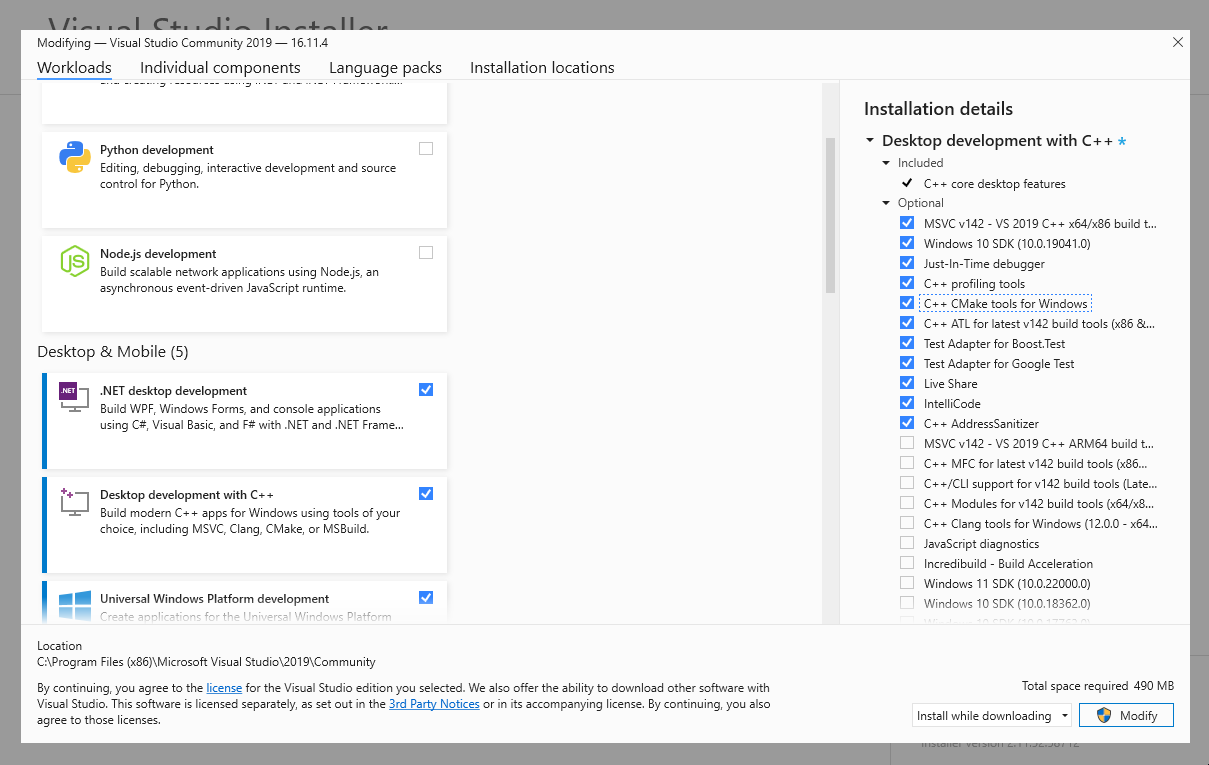
\includegraphics[width=0.85\textwidth]{./graf/vscmakeinstall.png}
\caption{Instalacja wsparcia systemu CMake w instalatorze środowiska Visual Studio}
\label{fig:vs-cmake-install}
\end{figure}

Po zweryfikowaniu instalacji wsparcia systemu CMake należy uruchomić środowisko Visual Studio, a następnie wybrać opcję Open local folder. Następnie należy wybrać główny folder projektu. Po otwarciu projektu i skończeniu generacji środowiska CMake należy zmienić opcję Select startup item na raymarcher.exe. Po wykonaniu powyższych kroków, projekt można budować oraz kompilować jak zwykły projekt środowiska Visual Studio.

\subsection{Instalacja wykorzystując narzędzie CMake}

\section{Sposób obsługi}
Po uruchomieniu program przedstawia prosty interfejs użytkownika. Cały
obszar okna wykorzystywany jest do wyświetlania renderowanego terenu.
Dodatkowo wewnątrz okna renderowany jest obszar zawierający pola
pozwalające na zmiane parametrów związanych z renderowaniem oraz generacją
terenu. Użytkownik ma możliwość poruszania kamerą korzystając z klawiszy W, S, A oraz D. Zmiana orientacji kamery jest możliwa poprzez poruszanie myszką gdy wyśnięty jest lewy przycisk myszki. Szczegółowe informacje dotyczące korzystania z interfejsu użytkownika można uzyskać naciskając przycisk Show UI Help. Program można zakończyć poprzez nmaciśnięcie przycisku Escape lub zamknięcie okna.

\begin{figure}
\centering
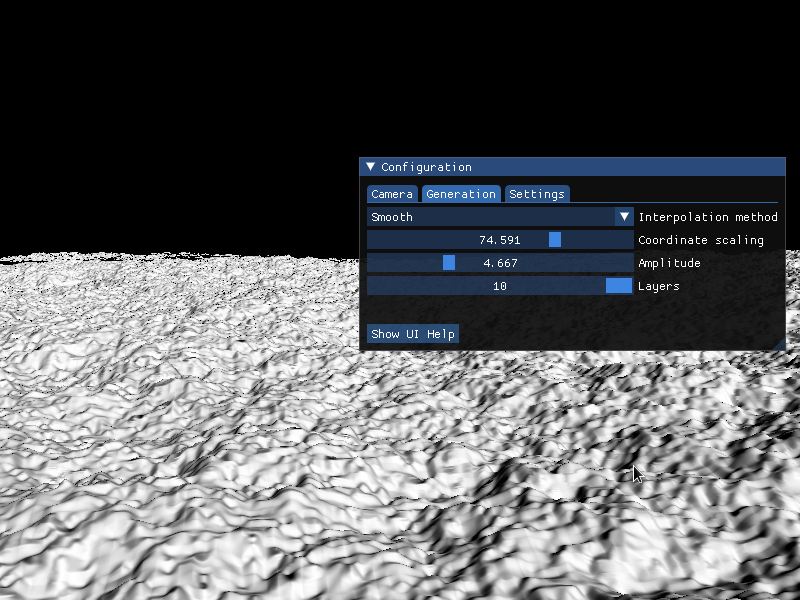
\includegraphics[width=0.5\textwidth]{./graf/ui.png}
\caption{Interfejs użytkownika}
\label{fig:ui}
\end{figure}


\section{Przykład działania}
do dodania po implementacji reszty programu.


\begin{itemize}
\item  wymagania sprzętowe i programowe
\item  sposób instalacji
\item  sposób aktywacji
\item  kategorie użytkowników
\item  sposób obsługi
\item  administracja systemem
\item  kwestie bezpieczeństwa
\item  przykład działania
\item  scenariusze korzystania z systemu (ilustrowane zrzutami z ekranu lub generowanymi dokumentami)
\end{itemize}

%%%%%%%%%%%%%%%%%%%%%
%% RYSUNEK Z PLIKU
%
%\begin{figure}
%\centering
%
\includegraphics[width=0.5\textwidth]{./graf/politechnika_sl_logo_bw_pion_pl.pdf}
%\caption{Podpis rysunku zawsze pod rysunkiem.}
%\label{fig:etykieta-rysunku}
%\end{figure}
%Rys. \ref{fig:etykieta-rysunku} przestawia …
%%%%%%%%%%%%%%%%%%%%%
%
%%%%%%%%%%%%%%%%%%%%%
%% WIELE RYSUNKÓW
%
%\begin{figure}
%\centering
%\begin{subfigure}{0.4\textwidth}
%    
\includegraphics[width=\textwidth]{./graf/politechnika_sl_logo_bw_pion_pl.pdf}
%    \caption{Lewy górny rysunek.}
%    \label{fig:lewy-gorny}
%\end{subfigure}
%\hfill
%\begin{subfigure}{0.4\textwidth}
%    
\includegraphics[width=\textwidth]{./graf/politechnika_sl_logo_bw_pion_pl.pdf}
%    \caption{Prawy górny rysunek.}
%    \label{fig:prawy-gorny}
%\end{subfigure}
%
%\begin{subfigure}{0.4\textwidth}
%    
\includegraphics[width=\textwidth]{./graf/politechnika_sl_logo_bw_pion_pl.pdf}
%    \caption{Lewy dolny rysunek.}
%    \label{fig:lewy-dolny}
%\end{subfigure}
%\hfill
%\begin{subfigure}{0.4\textwidth}
%    
\includegraphics[width=\textwidth]{./graf/politechnika_sl_logo_bw_pion_pl.pdf}
%    \caption{Prawy dolny rysunek.}
%    \label{fig:prawy-dolny}
%\end{subfigure}
%
%\caption{Wspólny podpis kilku rysunków.}
%\label{fig:wiele-rysunkow}
%\end{figure}
%Rys. \ref{fig:wiele-rysunkow} przestawia wiele ważnych informacji, np. rys. \ref{fig:prawy-gorny} jest na prawo u góry.
%%%%%%%%%%%%%%%%%%%%%


 
%% \begin{figure}
%% \centering
%% \begin{tikzpicture}
%% \begin{axis}[
%%     y tick label style={
%%         /pgf/number format/.cd,
%%             fixed,   % po zakomentowaniu os rzednych jest indeksowana wykladniczo
%%             fixed zerofill, % 1.0 zamiast 1
%%             precision=1,
%%         /tikz/.cd
%%     },
%%     x tick label style={
%%         /pgf/number format/.cd,
%%             fixed,
%%             fixed zerofill,
%%             precision=2,
%%         /tikz/.cd
%%     }
%% ]
%% \addplot [domain=0.0:0.1] {rnd};
%% \end{axis}
%% \end{tikzpicture}
%% \caption{Podpis rysunku po rysunkiem.}
%% \label{fig:2}
%% \end{figure}
